\subsection{Risk Evaluation}

\subsubsection{UI Mockup}


\begin{figure}[H]
\centering
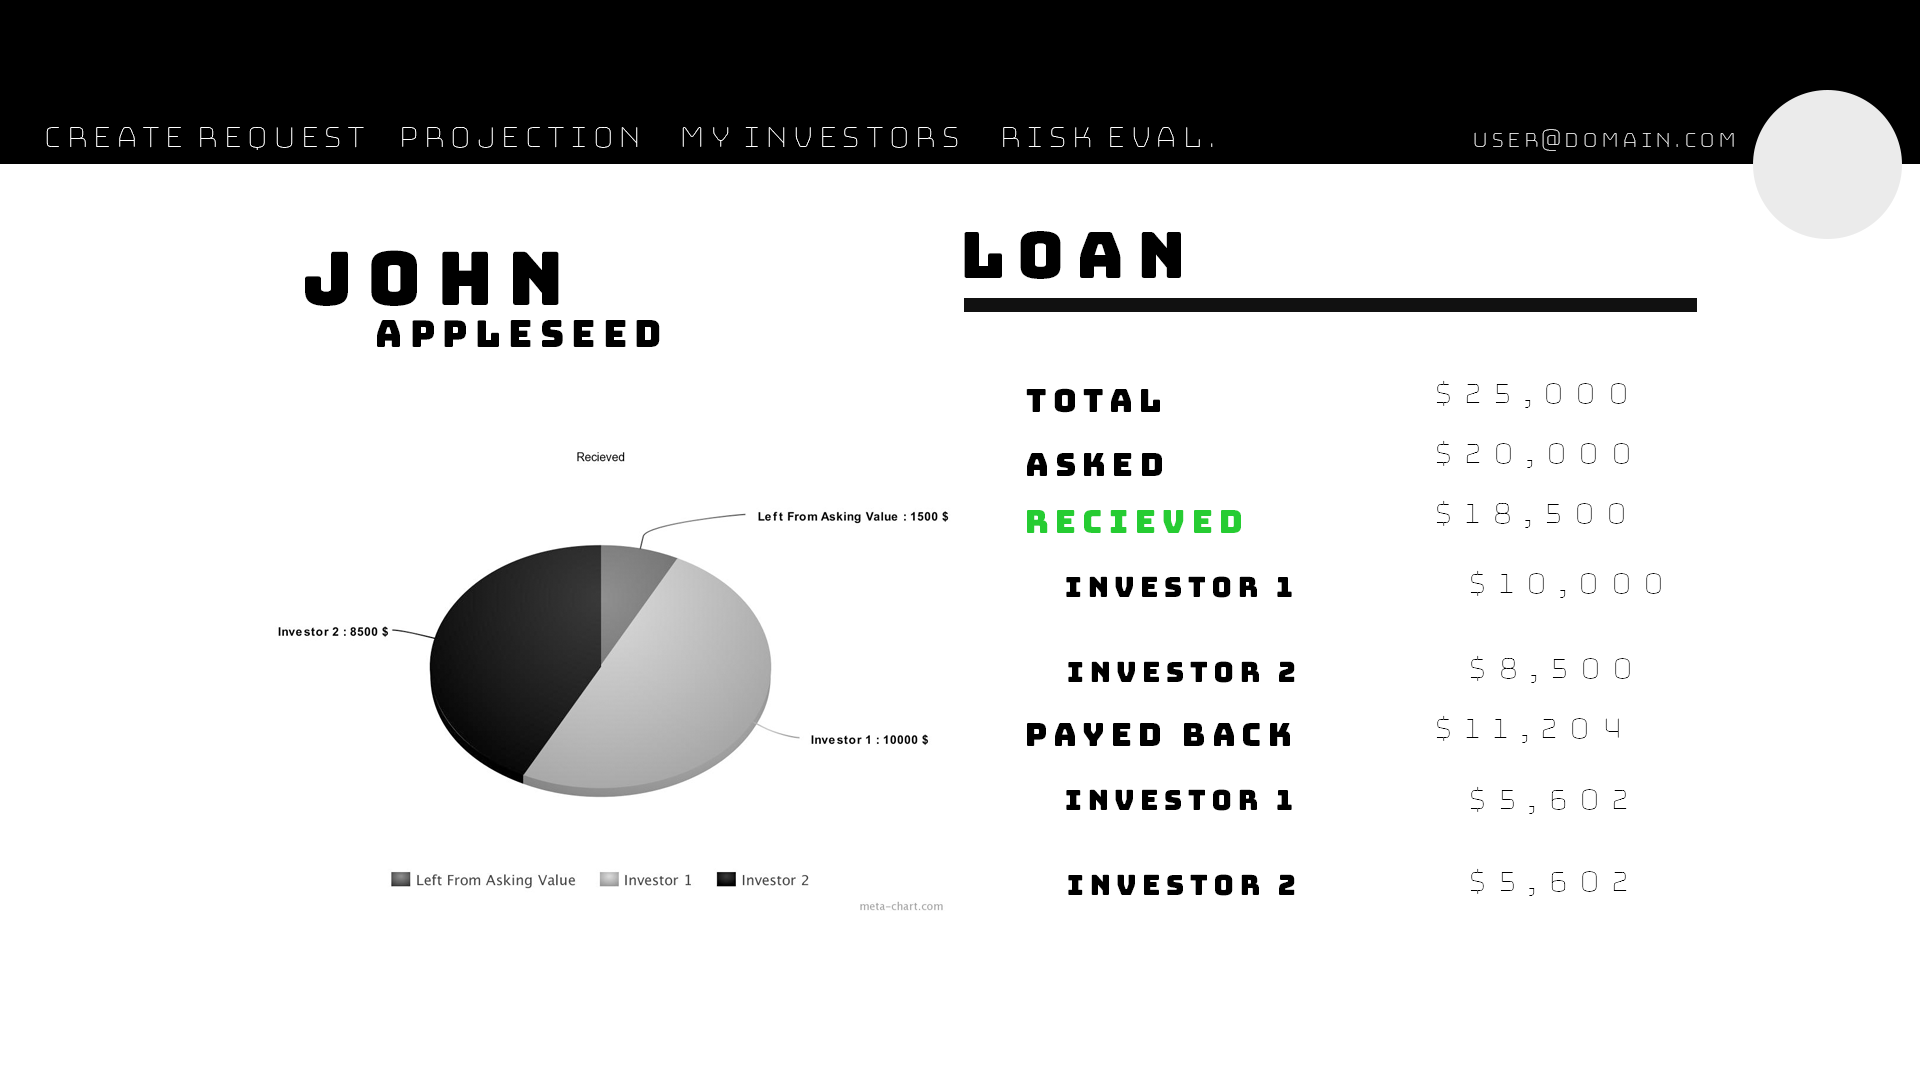
\includegraphics[width=\textwidth]{Account_Overview_Borrower}
\caption{Account overview page}
\end{figure}

\begin{figure}[H]
\centering
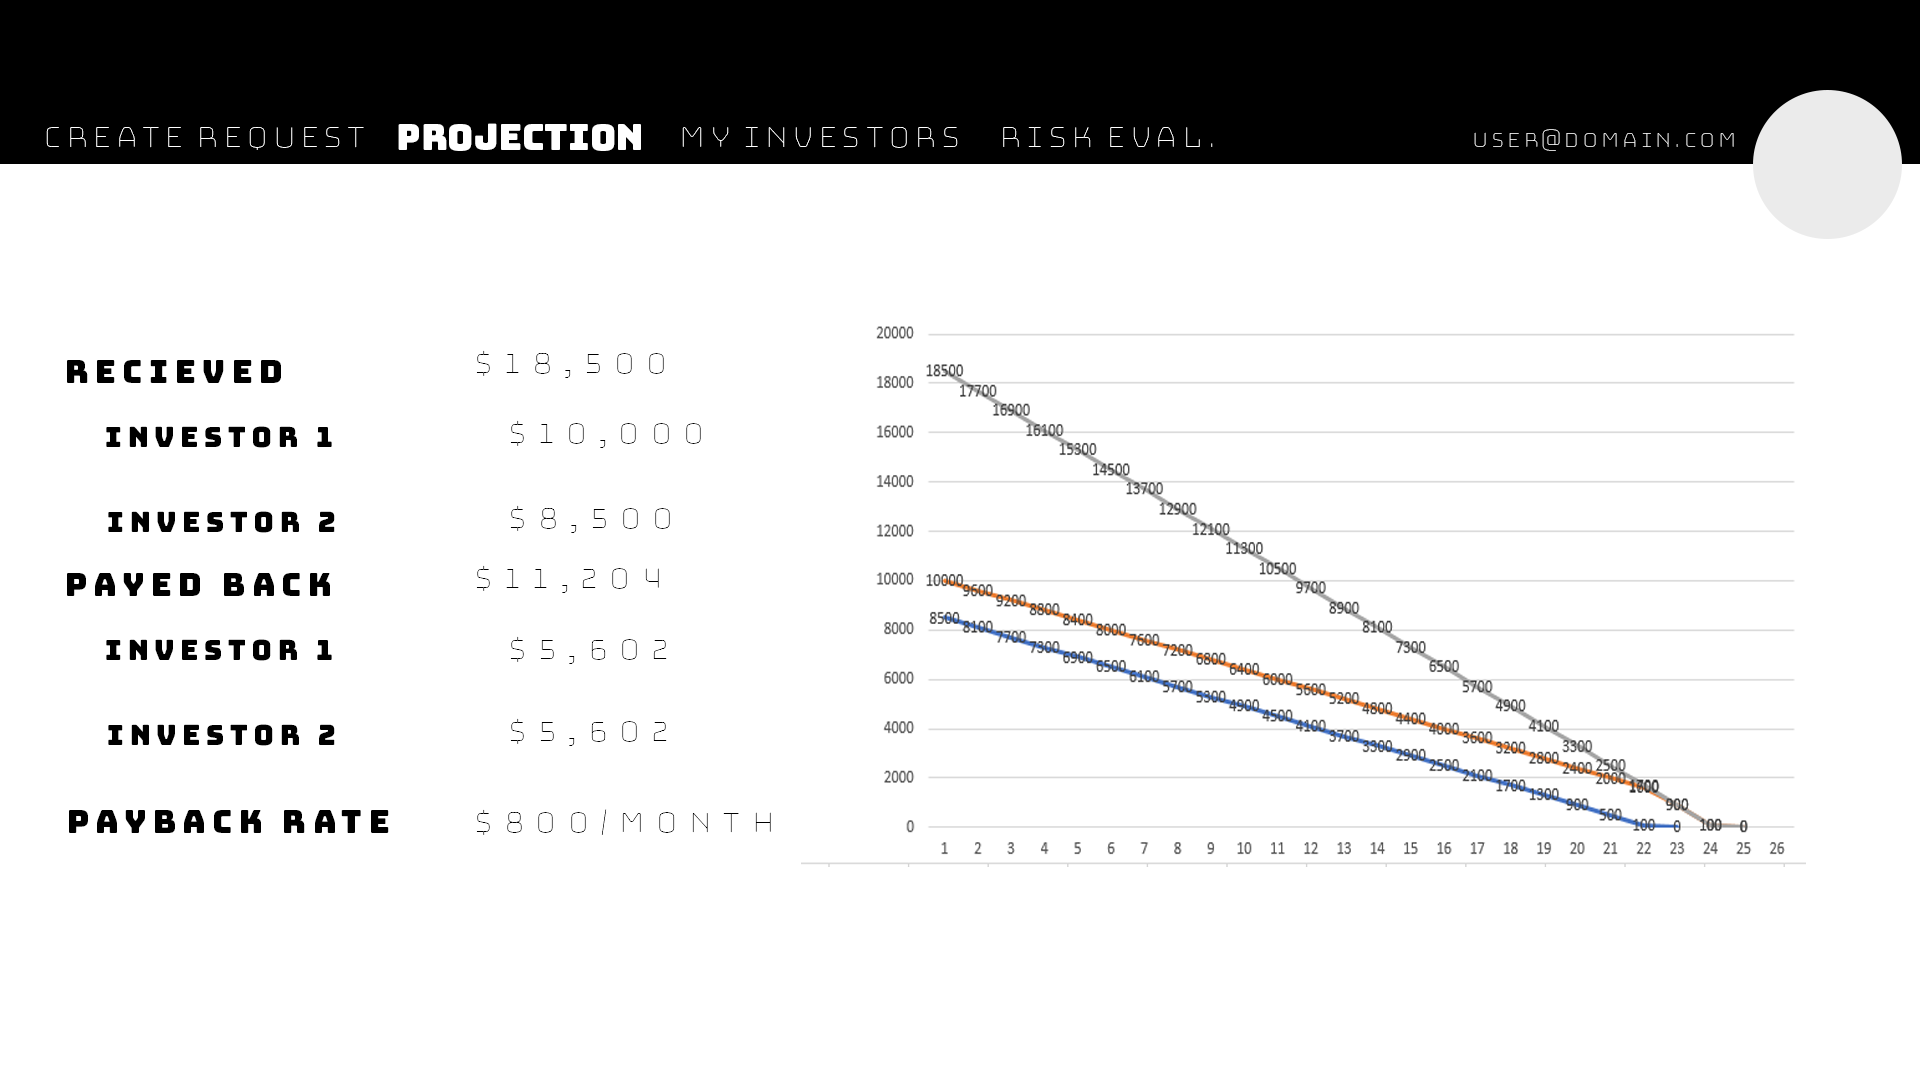
\includegraphics[width=\textwidth]{Loan_Projection_Borrower}
\caption{Loan Projection page}
\end{figure}

\begin{figure}[H]
\centering
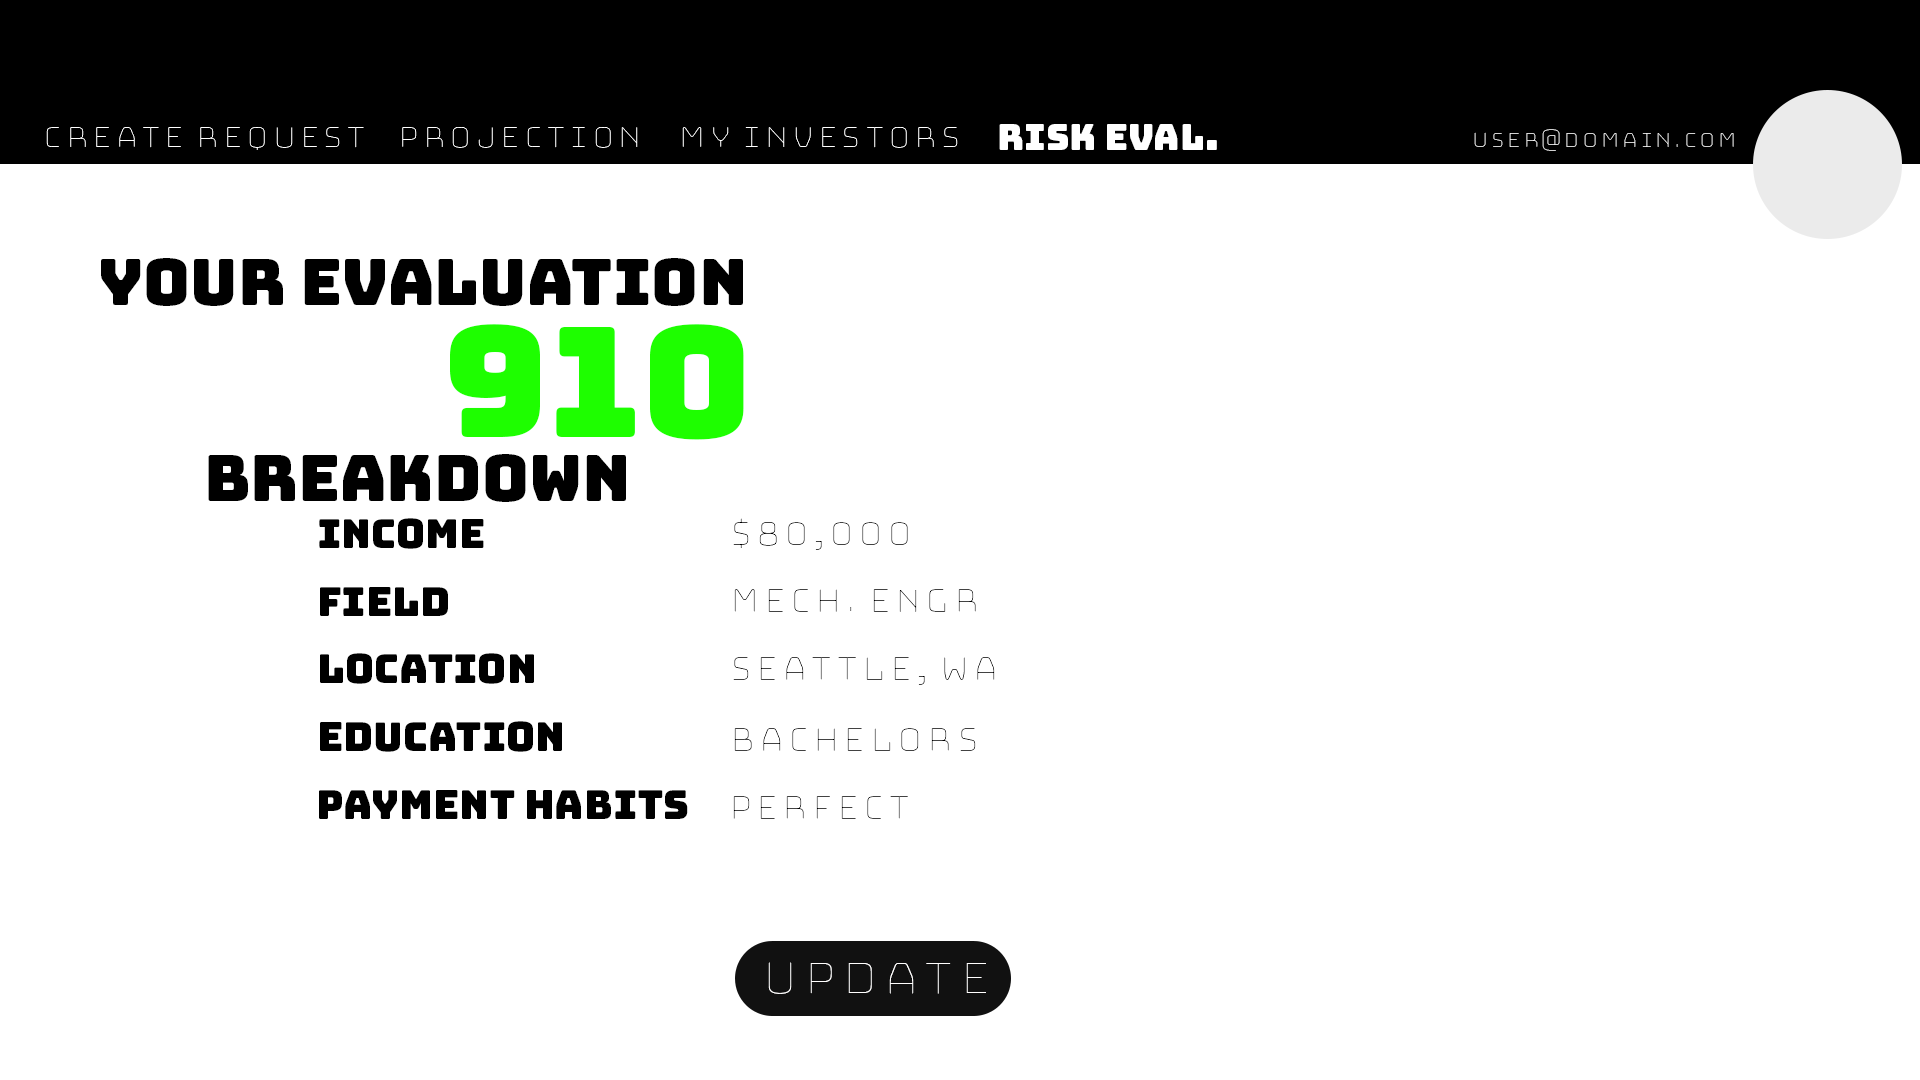
\includegraphics[width=\textwidth]{Risk_Evaluation_Overview_Borrower}
\caption{Risk Evaluation Overview}
\end{figure}

\begin{figure}[H]
\centering
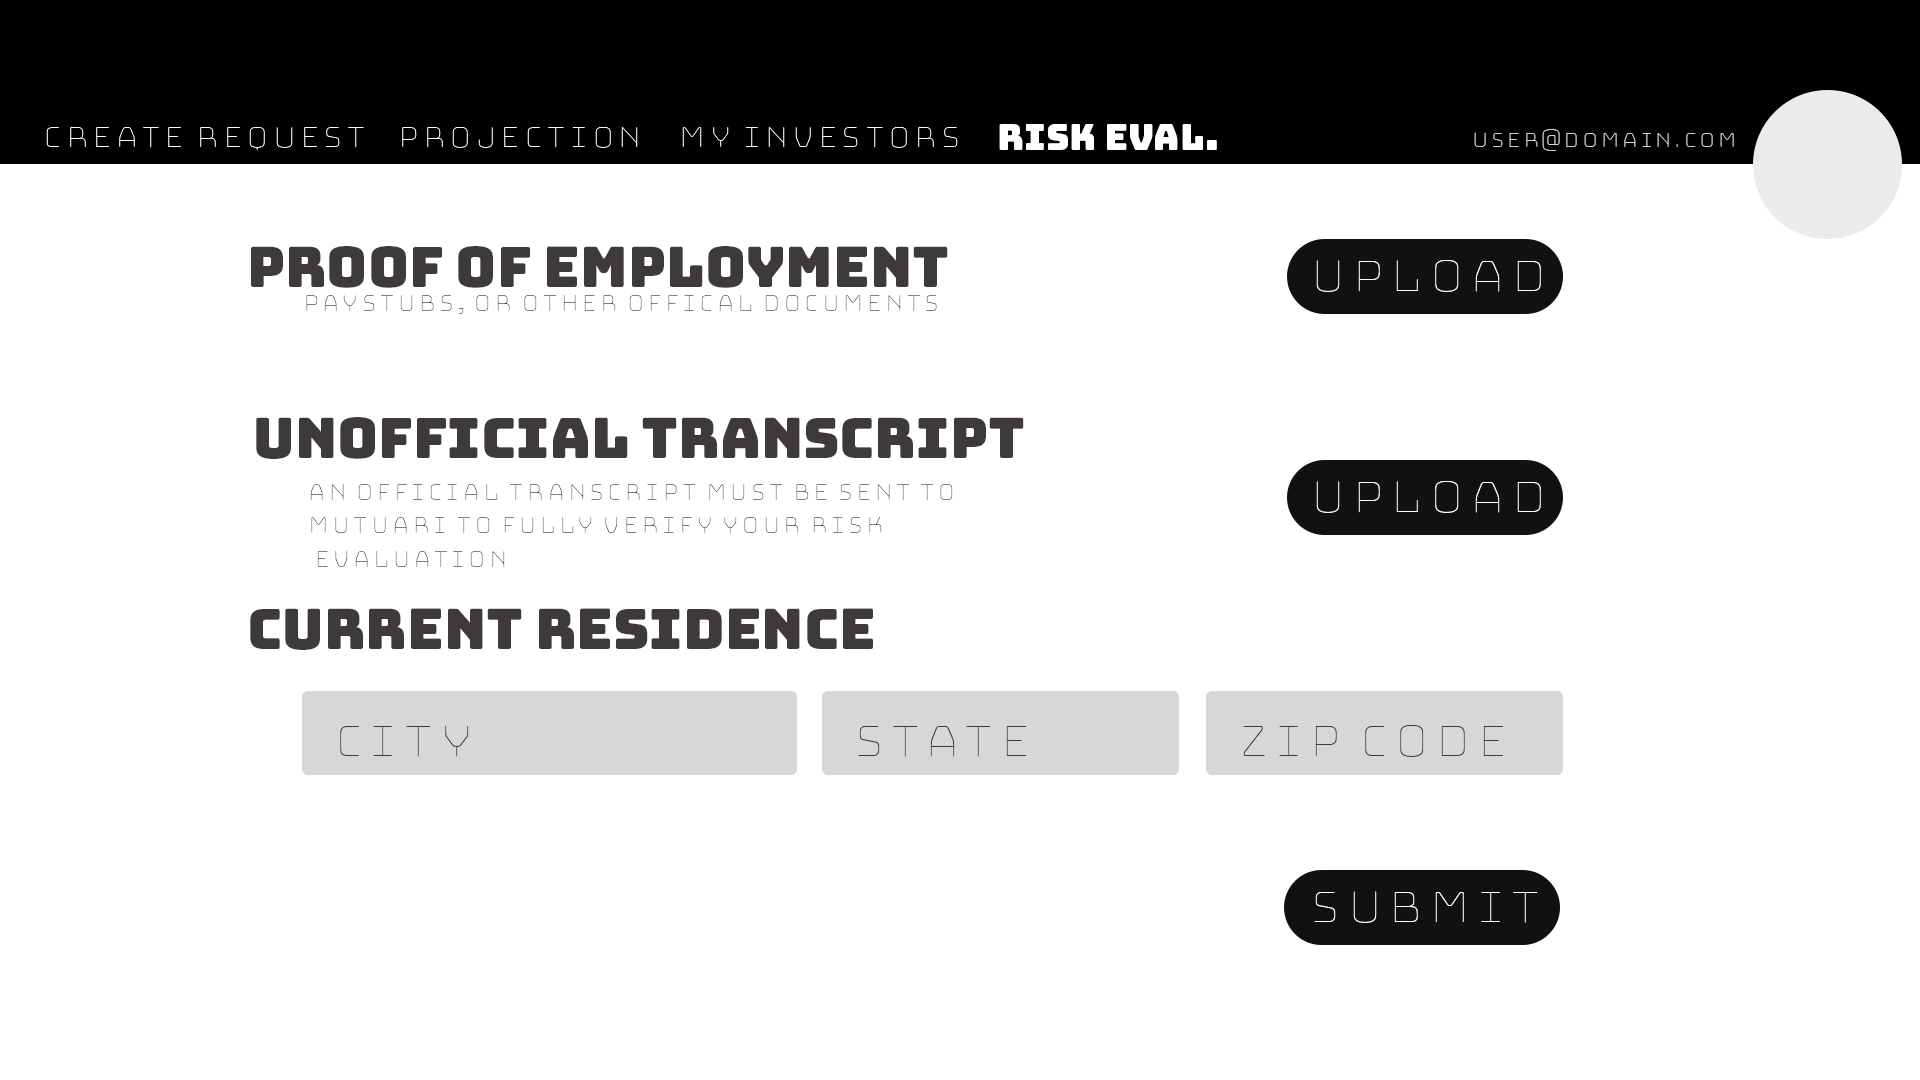
\includegraphics[width=\textwidth]{Risk_Evaluation_Input_Borrower}
\caption{Risk Evaluation Input}
\end{figure}



\subsubsection{UI Instructions}

\begin{enumerate}
	\item A Lender or Borrower accesses the Borrower's profile overview
	\item The lender can access the Borrower's profile overvie(Fig. 1), the Borrower's payoff projection(Fig. 2), and the Borrowers Risk Evaluation(Fig. 3)
	\item The Borrower can access the same as the lender, in addition to the Risk Evaluation Update page(Fig. 4) where they can upload additional information
\end{enumerate}
